\section{Distributed Memory}
\label{sec:mpi}

For a distributed memory implementation, The \textit{Message Passing Interface} (MPI) was used. With the sequential code having already suffered some changes and optimizations, the main problem consisted in the partitioning of the mesh. The obvious approach is one where each processor is assigned to a subset of the entire mesh, and is responsible for the application of both kernels to its subset. Communication is also required between each main loop iteration, since each process will require access to the values in the border of its subset, in order to compute its own values.

\subsection{Mesh Partitioning}
\label{subsec:mpi:partitioning}

In order to distribute processing payload across each process, the input mesh, and all of the data associated with it, also needs to be split into partitions. A mesh partitioning algorithm is required. This algorithm must generate $P$ disjoined partitions (where $P$ is the number of processors available), each to be assigned to a different processor. Some additional data is also required for each partition, so that information about how each partition connects to the others is kept, to allow communication to be done correctly.

\subsubsection{Research in Mesh Partitioning}
\label{subsubsec:mpi:partitioning:research}

Mesh partitioning is currently an actively researched topic, with some projects and libraries begin already available that help with the understanding of how a mesh (or more generically, a graph) can be partitioned in ways to optimize certain aspects like load balancing, communication balancing or partitioning overhead. For instance, in \cite{metis}, a library called \texttt{Metis} is presented whose purpose is precisely this problem. Other works found for this topic included \cite{gilbert1995, walshaw2000}.

However, given the time constraints of this project, and since the priority was to have a functional algorithm rather than an optimal one, it was decided not to attempt an approach involving \texttt{Metis} or any other researched work. Actually, the method used to partition the mesh is quite naive, as shown in \cref{subsubsec:mpi:partitioning:method}.

\subsubsection{Partitioning Methodology}
\label{subsubsec:mpi:partitioning:method}

he algorithm created to partition the mesh works by dividing it in slices by the horizontal coordinate of each cell. Givem a mesh with a total of 100 cells, and a pool of $P$ processes, the mesh is divided into $P$ partitions, each with exactly $N=100/P$ cells, differing by at most one cell when they cannot be evenly divided. By ordering the cells based on their $x$ coordinate, they are sequentially assigned to each process, in such a way that the first process receives the first $N$ cells of the set, and so on.

\begin{figure}[!htp]
	\begin{subfigure}[b]{0.5\columnwidth}
		\centering
		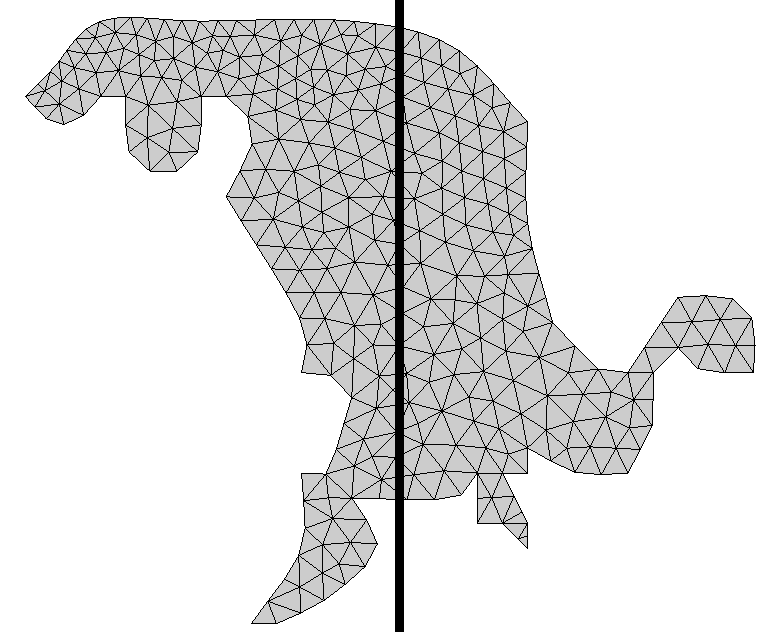
\includegraphics[width=\columnwidth]{foz_p2_msh}
		\caption{2 partitions}
		\label{fig:foz_p2_msh}
	\end{subfigure}%
	\begin{subfigure}[b]{0.5\columnwidth}
		\centering
		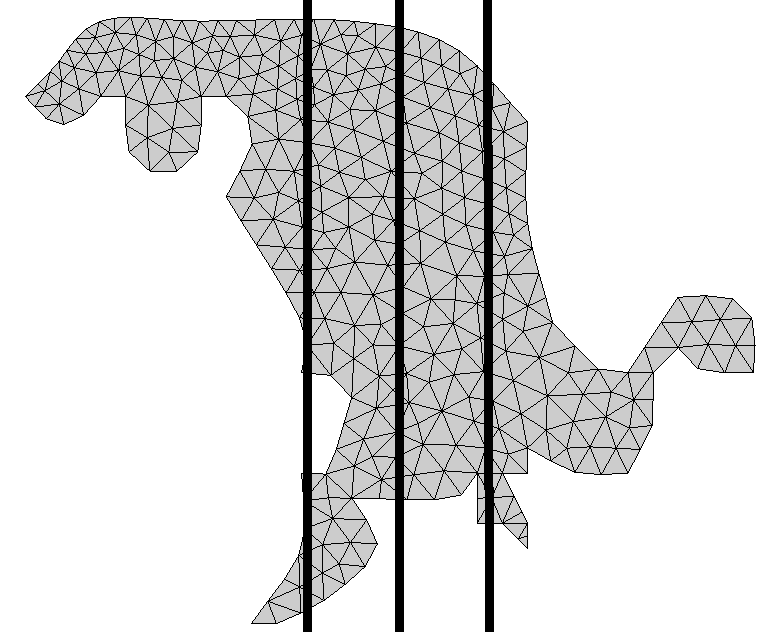
\includegraphics[width=\columnwidth]{foz_p4_msh}
		\caption{4 partitions}
		\label{fig:foz_p4_msh}
	\end{subfigure}%

	\caption{Mesh partitioning illustration}
	\label{fig:partitioning}
\end{figure}

With this partitioning method, communication is also greatly simplified, as it is guaranteed that every partition will have a left and a right neighbor. It is also assumed that the width of the global mesh is big enough so that there are never processes with 0 cells assigned, which would break communication. Since a common mesh usually contains at least thousands of cells, this should not be an issue.
On the other hand, the partitioning and assignement of the cells is done sequentially, and will increase preparation time.

\subsection{Communication Analysis}
\label{subsec:mpi:comm}

When computing the flux for a given edge, the pollution values of both adjacent cells are required. Until now, only one divergent case existed, when the edge was in the border of the mesh. With the addition of partitioning, a new divergence is created, when the edge is not in the border of the global mesh, but in the border of the local partition, meaning that one of its adjacent cells was assigned to a different partition.

A communication step is required at this point, so that each edge in the local border (the border that connects to another partition, not the global mesh border) receives the corresponding values from the neighbor partition 

This communication step was introduced at the beginning of the main loop, and consists of two smaller steps, one for left communication, and one for right communication.
Each iteration, every process starts by communicating the left border values, which were previously indexed in the preparation stage, to its left neighbor. Asynchronously with that task, it receives an equivalent message from the right neighbor, which is also at the same step. After both tasks, the direction of communication is reversed, and the right border values are sent to the right neighbor of each partition.

Only after all communication is done for this process can it continue to the main kernels of the loop. This introduces a large overhead, as it will most likely require a network transfer if the neighbor partition is located in a different machine. This overhead may become a huge bottleneck for the loop, especially for smaller inputs, where the time spent in the kernels is small enough to make the partitioning and communication occupy a large percentage of the program.

An alternative could consist in making the communication an asynchronous task, allowing the flux for inner edges to be computed while the communication is taking place, since they don't depend on the values to be received. Again, due to time constraints, it was not possible to better analyse this solution.

\subsection{Load Balance}
\label{subsec:mpi:load}

\todorev{Last revised on Sat, June 30 at 23:15 by pfac}

With the naive partitioning strategy used, load balance becomes a problem.
The computation itself is actually well balanced, since it is assured that every partition has the same amount of cells (differing at most by one). The problem is in the border between those partitions.
With the division by the horizontal coordinate being used, it becomes obvious that the size of the border between partitions becomes extremely dependant on the format of the mesh itself.
Other approaches, already mentioned in \cref{subsubsec:mpi:partitioning:research} attempt to deal with this, and produce partitions that minimize the size of the border.

The drawback of not controlling border sizes comes at the communication step.
Not only a different partitioning solution could minimize the border, thus minimizing the amount of data transfered, it can also happen that different partitions have very different border sizes, compromising communication balance.

\todonaps{Anhe? Esta última frase faz grande sentido para mim.}

